In classical physics, electric conduction is described as the motion of charged particles under the influence of an external field. According to Newtonian mechanics, when an electric field is applied across a conductor, free electrons accelerate in the direction opposite the field, producing a current. The current density is proportional to the applied field, as captured by Ohm’s law. Scattering from impurities or lattice vibrations introduces resistance, and the microscopic origin of conductivity is attributed to the mean free path and average velocity of the charge carriers.

This model explains why metals conduct and insulators do not by appealing to the number of mobile electrons. A material with more conduction electrons, or fewer collisions, should exhibit lower resistance. However, this account fails to explain several observations. The resistivity of some metals decreases monotonically with temperature, while in others it saturates. Pure crystalline insulators show negligible conduction even though electrons are present. Most strikingly, two materials with similar atomic composition can differ dramatically in electrical behavior. These inconsistencies point to limitations in the classical picture.

Quantum theory redefines the conditions for electrical conduction. In contrast to classical models, electrons in a solid do not behave as free particles moving through a continuous background. Instead, their behavior is governed by quantum statistics and the discrete structure of available energy levels. Each electron occupies a single-particle quantum state, and no two electrons may share the same state — a constraint imposed by the Pauli exclusion principle.

At zero temperature, electrons occupy the lowest available energy levels, filling all states up to a well-defined maximum energy. This threshold is called the \emph{Fermi energy}. It represents the top of the occupied spectrum in the ground state and serves as the reference point for determining whether an electron can respond to an external field. For conduction to occur, an electron near this boundary must be able to transition to an adjacent, unoccupied state.

In quantum systems, such transitions require the presence of accessible states arbitrarily close in energy to the occupied ones. If these states exist, an applied field perturbs the electron distribution near the Fermi surface, inducing current. If no such nearby states are available — either because all are filled or because the next states lie across a finite energy gap — the field cannot induce a first-order response. The system remains non-conductive.

This obstruction is not caused by spatial localization or mechanical confinement. It is a consequence of spectral structure: the organization of energy levels and the exclusion constraints that govern their occupancy. A material may contain delocalized electrons, yet fail to conduct if their quantum states are completely filled. The defining criterion is the existence of a \emph{partially filled band} — a continuous set of states near the Fermi energy that electrons can access without violating exclusion.

This distinction separates conductors from insulators. In metals, the Fermi level lies within a band, allowing infinitesimal adjustments in electron momentum and enabling conduction. In insulators, the Fermi level falls inside a band gap: a region devoid of permissible states. No electrons can respond to the field unless they are excited across the gap. Semiconductors occupy an intermediate regime, where the gap is small enough to be overcome thermally or chemically. In all cases, the decisive factor is not the number of electrons present, but the spectral topology near the Fermi energy — the structure of quantum states at the point where occupancy terminates.

This view resolves several paradoxes. Materials with identical valence electron counts can behave as metals or insulators depending on lattice symmetry and orbital structure. Even small changes in atomic arrangement or spin-orbit coupling can close or open a gap. The conventional measure of conduction — electrons per atom — is not predictive. Instead, conduction reveals how the spectrum is organized, and whether the system admits low-energy excitations compatible with the field.

In \textbf{crystalline solids} — materials whose atoms are arranged in a regular, repeating pattern — electrons experience a periodic potential generated by the lattice structure. This periodicity constrains the solutions to the Schrödinger equation, leading to wavefunctions of the form
\[
\psi_{n\mathbf{k}}(\mathbf{r}) = e^{i\mathbf{k} \cdot \mathbf{r}} u_{n\mathbf{k}}(\mathbf{r}),
\]
where \( u_{n\mathbf{k}}(\mathbf{r}) \) is periodic with the lattice and \( \mathbf{k} \) is the crystal momentum. These solutions are known as \emph{Bloch waves}. Due to the discrete translational symmetry of the lattice, the set of physically distinct momenta is restricted to a finite region called the \emph{Brillouin zone}, which has the topology of a torus in two or more dimensions.

The energies associated with Bloch states form continuous intervals called \emph{bands}, separated by \emph{band gaps} — regions of energy for which no eigenstates exist. At zero temperature, electrons fill the lowest available energy states, completely occupying bands up to the \emph{Fermi energy}, the highest occupied level. Whether or not a material conducts electricity depends on the presence of accessible quantum states near this energy.

In a \textbf{metal}, the Fermi energy lies within a partially filled band. This means that, within an arbitrarily small energy interval, there exist unoccupied states into which electrons can transition. As a result, an external electric field causes a redistribution of occupation within this band. The current is carried by electrons near the Fermi surface — states that can shift slightly in momentum while remaining in the same band. Although scattering from phonons or impurities can limit the magnitude of conduction, it does not eliminate the overall response.

In a \textbf{band insulator}, the Fermi energy lies inside a band gap: a region of forbidden energy that separates a fully filled \emph{valence band} from an empty \emph{conduction band}. Since all states near the Fermi level are either fully occupied or entirely absent, no electronic transitions can occur in response to weak fields. Conduction is only possible if electrons are excited across the gap, which requires energy on the order of several electron-volts. At low temperatures and in the absence of strong perturbations, the material remains inert.

A \textbf{semiconductor} also possesses a gap between filled and empty bands, but the gap is significantly smaller — typically between 0.1 and 2 electron-volts. At finite temperatures, some electrons can be thermally excited from the valence band into the conduction band, generating mobile charge carriers. In addition, the electrical properties of semiconductors can be tuned by introducing dopants — impurities that shift the chemical potential into one of the bands, increasing the carrier concentration. These features make semiconductors responsive to temperature, chemical environment, and external fields, enabling their widespread use in electronic and optoelectronic devices.

The conventional classification of electronic materials — into \textbf{metals}, \textbf{semiconductors}, and \textbf{insulators} — is determined by the position of the Fermi level relative to the energy bands. This framework describes whether low-energy excitations are available to carry current: metals have partially filled bands, insulators have completely filled bands with a finite gap to the next available states, and semiconductors occupy an intermediate regime with a small, thermally bridgeable gap. While this classification successfully predicts electrical behavior, it accounts only for the \emph{energy spectrum} of the system. It does not capture how the quantum wavefunctions are structured across momentum space. Two materials may exhibit identical band energies and yet differ fundamentally in their quantum phase. A complete description requires not only knowledge of the spectrum, but of the global organization of the eigenstates.

In mathematics, \textbf{topology} refers to the study of properties that are preserved under continuous deformations. Two objects are topologically equivalent if one can be transformed into the other without cutting or gluing. A sphere and a cube are equivalent in this sense; a sphere and a torus are not. Topological classification assigns discrete labels to such global properties — labels that remain unchanged under smooth variation. When applied to quantum systems, topology concerns the structure of wavefunctions across the Brillouin zone. These wavefunctions form continuous families of states, and the way they are “glued together” over momentum space can be trivial or twisted. This distinction, invisible to ordinary band diagrams, gives rise to a richer taxonomy of phases — \emph{topological phases} — which remain sharply distinct as long as certain symmetries and energy gaps are preserved.


In crystalline solids, the topological structure refers not to the real-space geometry of the material, but to the global organization of the electronic wavefunctions over the Brillouin zone. The occupied states at each momentum form a smooth family — a \emph{vector bundle} over the Brillouin zone. If a smooth, continuous labeling of these states exists globally, the bundle is trivial. If singularities or twisting obstruct such a labeling, the system is said to have nontrivial topology.

Topological features of the wavefunctions are invisible to conventional band theory, which sees only the energies. Two systems can have identical energy bands but differ in the global structure of their quantum states. This difference is characterized by discrete quantities called \emph{topological invariants}, which remain unchanged under smooth deformations that preserve the energy gap and symmetries.

The nature of the invariant depends on dimensionality and symmetry. In two-dimensional systems that break time-reversal symmetry — such as in the quantum Hall effect — the topology is captured by an integer known as the \emph{Chern number}, which counts how the wavefunctions twist across the Brillouin zone. In time-reversal-invariant systems, the classification is subtler: the relevant invariant is binary, distinguishing between trivial and nontrivial phases, and is captured by a \(\mathbb{Z}_2\) index.

Topological insulators often emerge through \emph{band inversion}. In ordinary materials, states derived from low-angular-momentum atomic orbitals lie below those from higher angular momentum. Strong spin-orbit coupling can reverse this ordering, causing states that should belong to the conduction band to sink below the valence band. This inversion alters the topology of the occupied wavefunctions, resulting in a topologically nontrivial phase.

At the boundary between two regions with different topological classifications, the energy gap must close locally. The transition between distinct global structures cannot happen smoothly while maintaining a finite gap. As a result, electronic states appear confined to the boundary — states that traverse the bulk energy gap and are robust against disorder. This phenomenon is known as \textbf{bulk-boundary correspondence}.

In many topological insulators, the relevant distinction is protected by time-reversal symmetry. This symmetry implies that for every electronic state with a given spin and momentum, there exists a partner state with opposite spin and opposite momentum at the same energy. These pairs form what are known as Kramers doublets. On the boundary, this symmetry enforces that electrons with opposite spins propagate in opposite directions. Scattering between these modes requires both a reversal of spin and momentum — a process that is forbidden unless time-reversal symmetry is broken. As a result, non-magnetic disorder, surface roughness, and other imperfections do not localize these boundary states. They remain extended, conducting channels pinned to the edge or surface.

Although topological insulators support boundary conduction, their interiors remain fully gapped. The bulk spectrum is indistinguishable from that of an ordinary insulator: no low-energy states are available, and no current flows under typical conditions. What distinguishes these materials is not the existence of surface states alone, but the fact that those states are guaranteed by the topology of the underlying quantum structure.

The presence of boundary states in topological insulators has been confirmed experimentally. In materials such as Bi\(_2\)Se\(_3\), Bi\(_2\)Te\(_3\), and Sb\(_2\)Te\(_3\), angle-resolved photoemission spectroscopy (ARPES) provides direct evidence of surface states traversing the bulk energy gap. ARPES is a momentum-resolved technique that maps the energy of electrons as a function of their crystal momentum. In topological materials, these measurements reveal conducting states localized at the surface that connect the valence and conduction bands — a signature of the nontrivial topological phase. The resulting dispersion curves show linear energy–momentum relations resembling those of massless Dirac fermions, centered at time-reversal-invariant momenta in the Brillouin zone.

Transport measurements further support this characterization. When the bulk is sufficiently insulating, the electrical conductance measured at low temperatures remains finite and reflects contributions from surface channels. These conducting modes are stable across a range of sample thicknesses, geometries, and surface treatments. They persist even when the crystal is cleaved or exposed to ambient conditions, so long as time-reversal symmetry is preserved. Magnetotransport experiments reveal weak anti-localization effects and spin-momentum locking, consistent with theoretical models of helical edge states.

These observations cannot be explained by ordinary surface effects such as dangling bonds, surface reconstructions, or impurity bands. Such features depend sensitively on chemical termination and sample preparation, and typically vary between experiments. By contrast, the conducting surface states observed in topological insulators display a fixed, reproducible structure: they appear at well-defined momentum points, connect the bulk valence and conduction bands, and persist across a wide range of materials and conditions. ARPES consistently reveals Dirac-like surface bands spanning the bulk energy gap, regardless of sample thickness, cleavage direction, or surface treatment. Their stability under nonmagnetic disorder and their resistance to localization confirm that these states are not surface anomalies. Instead, they are required by the topological structure of the bulk wavefunctions. According to bulk-boundary correspondence, when two regions differ in topological invariant — as a nontrivial insulator meets vacuum — the boundary must host conducting states. These states are remarkably insistent: they cannot be eliminated by any local modification unless a protecting symmetry is broken or the bulk gap closes. Their existence is not contingent on surface chemistry or atomic detail. Rather, it reflects a nonlocal constraint — a continuity condition imposed by the quantum geometry of the entire system.

The physical consequences of this protection are significant. Because the surface modes are stable against a broad class of perturbations, topological insulators provide a platform for low-dissipation electronic devices. Scattering by non-magnetic disorder does not localize the boundary states, and backscattering is suppressed by symmetry constraints. This makes them attractive candidates for interconnects and surface-conduction components that remain reliable under fabrication imperfections and environmental variation.

More speculative — but deeply studied — are the implications for quantum information. When topological insulators are brought into contact with superconductors, the resulting interface can host quasiparticles with non-Abelian exchange statistics. These excitations, which obey different algebraic rules than bosons or fermions, are of interest for topological quantum computation. In such architectures, quantum information is encoded in the collective state of multiple quasiparticles, and operations correspond to their braiding in space. Because the resulting transformations depend on topology rather than local details, they are intrinsically fault-tolerant under a wide class of errors.

These applications remain under development, and experimental realization of non-Abelian quasiparticles in topological insulators is not yet definitive. Nonetheless, the theoretical infrastructure is robust, and related phenomena have been reported in engineered heterostructures involving superconductors and topological materials. The combination of stable conduction, symmetry-protected surface physics, and the possibility of coupling to exotic quantum phases makes topological insulators a focal point of both foundational and applied research in condensed matter physics.

\vspace*{\fill}
\begin{center}
\begin{minipage}{0.8\textwidth}
\begin{tcolorbox}[colback=gray!10!white, colframe=black!50!white, sharp corners, boxrule=0.3pt, width=0.9\textwidth, enhanced]
\small
\textbf{Some Jokes for a Topologist}

A man comes to the doctor with a bandage wrapped around his leg. The doctor asks, "What happened?" The man says, "I hurt my head." The doctor looks confused — "Then why is the bandage on your leg?" The man shrugs: "It slipped."

\vspace{1em}

Two topologists are trying to open a can of beans in a hotel room. One tries smashing it, stabbing it — nothing works. The other sits down, calculates carefully on paper, walks over confidently, and instantly disappears inside the can. From within, a voice shouts: "I must have gotten the sign wrong."

\vspace{1em}

A coconut is just a nut.

\vspace{1em}

Q: What does the B stand for in Benoit B. Mandelbrot?\\
A: Benoit B. Mandelbrot.

\vspace{1em}

Q: What's an anagram of Banach–Tarski?\\
A: Banach–Tarski Banach–Tarski.
\end{tcolorbox}
\end{minipage}
\end{center}
\vspace*{\fill}

\newpage
\thispagestyle{empty}
\begin{figure}[p]
\centering
\fbox{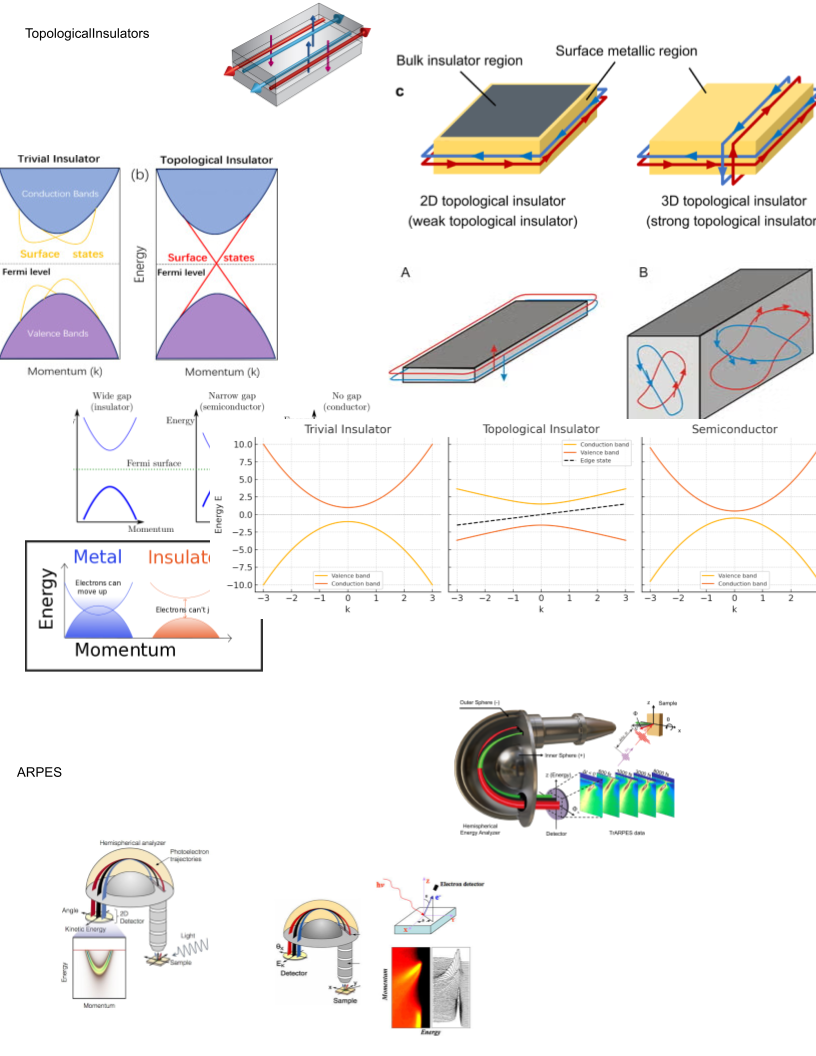
\includegraphics[width=\textwidth,height=\textheight,keepaspectratio]{02_TopologicalInsulators/topological.png}}
\end{figure}
\clearpage